% ══════════════════════════════════════════════════════════════
% CAPÍTULO — ENTORNO EMPRESARIAL
% Título de tesis: INTELIGENCIA ELECTORAL CON LLM: MINERÍA DE
% SENTIMIENTOS Y DETECCIÓN DINÁMICA DE TEMAS RELEVANTES PARA
% ANALIZAR LA PERCEPCIÓN ACTUAL PROYECTADA POR LOS MEDIOS DE
% COMUNICACIÓN EN ECOSISTEMAS DIGITALES
% Período de datos: enero–mayo 2026
% Fuentes: YouTube (transcripciones), X/Twitter (tweets),
%           portales de noticias (scraping web), TikTok
% ══════════════════════════════════════════════════════════════

\chapter{Entorno Empresarial}

\section{Descripción del contexto de aplicación}

\subsection{Reseña histórica y actividad}

El Jurado Nacional de Elecciones (JNE) es el organismo constitucional autónomo del Estado peruano encargado de administrar justicia en materia electoral, fiscalizar la legalidad del ejercicio del sufragio y de la realización de los procesos electorales, de referéndum y de otras consultas populares \parencite{ent_jne2023institucional}. Fue creado mediante la Constitución Política de 1933 y reafirmado como organismo autónomo por la Constitución vigente de 1993, siendo hoy uno de los tres organismos electorales del sistema democrático peruano, junto a la Oficina Nacional de Procesos Electorales (ONPE) y el Registro Nacional de Identificación y Estado Civil (RENIEC).

En el marco de los procesos electorales, la percepción que los medios de comunicación proyectan sobre los candidatos, partidos políticos y propuestas programáticas se construye y transforma principalmente a través del ecosistema digital. Las plataformas de noticias digitales, X (antes Twitter), YouTube y TikTok se han consolidado como los principales canales de difusión de contenido mediático durante las campañas electorales peruanas. Sin embargo, el análisis sistemático y automatizado de esta cobertura —en términos de su tono, encuadre y temática— ha sido hasta la fecha un reto técnico sin resolver a escala institucional.

La presente investigación se desarrolla como un proyecto académico aplicado orientado al análisis automatizado de la percepción proyectada por los medios de comunicación en ecosistemas digitales peruanos durante el proceso electoral. Para ello, se trabaja con un equipo multidisciplinario conformado por analistas políticos, especialistas en NLP e ingenieros de datos, cuyo interés es evaluar la viabilidad de un sistema automatizado de inteligencia electoral basado en Modelos de Lenguaje de Gran Escala (LLMs) sobre un corpus recolectado entre enero y mayo de 2026.

\subsection{Descripción de la organización}

\subsubsection{Organigrama del equipo de investigación aplicada}

El equipo de trabajo vinculado al desarrollo e implementación del sistema de inteligencia electoral propuesto en esta tesis está conformado por los siguientes roles, cuya estructura jerárquica se representa en la Figura \ref{fig:organigrama_equipo}.

\begin{itemize}
    \item \textbf{Director del Proyecto}: Responsable de la visión estratégica, la definición de los objetivos del sistema y la validación de los resultados desde una perspectiva de ciencia política y comunicación mediática. Coordina con los organismos electorales y los medios de comunicación interesados en el producto final.

    \item \textbf{Líder de Ciencia de Datos / NLP}: Diseña la arquitectura del pipeline de procesamiento de lenguaje natural, selecciona y ajusta los modelos LLM utilizados, y supervisa la calidad de los análisis de sentimientos y detección de temas sobre el corpus multimodal.

    \item \textbf{Ingeniero de Datos}: Responsable de la ingesta, almacenamiento y preprocesamiento de los datos multimodales en tiempo real. Gestiona los scrapers de noticias, las conexiones con las APIs de plataformas digitales (TwitterAPI.io), las herramientas de descarga y transcripción de contenido audiovisual (yt-dlp) y los sistemas de base de datos.

    \item \textbf{Analista Político Electoral}: Experto en el contexto político peruano y en la cobertura mediática electoral que valida cualitativamente los resultados del sistema, define los criterios de relevancia temática y asegura que los indicadores generados sean interpretables y útiles para la toma de decisiones.

    \item \textbf{Desarrollador de Visualización}: Diseña e implementa los dashboards interactivos que permiten explorar los resultados del sistema en tiempo real, así como los reportes automáticos generados al cierre de cada jornada electoral, incluyendo vistas comparadas por fuente mediática.

    \item \textbf{Especialista en Ética e Integridad Electoral}: Supervisa que el sistema opere dentro de los marcos legales y éticos aplicables, previene el uso indebido de los resultados y asegura la privacidad y anonimización de los datos ciudadanos procesados.
\end{itemize}

\begin{figure}[!ht]
    \begin{center}
        \includegraphics[width=0.82\textwidth]{2.5/figures/organigrama_equipo.jpg}
        \caption[Organigrama del equipo de investigación del sistema de inteligencia electoral]{Organigrama del equipo de investigación y desarrollo del sistema de inteligencia electoral basado en LLMs, mostrando la jerarquía y relaciones entre los roles definidos.\\
            Fuente: Elaboración propia.}
        \label{fig:organigrama_equipo}
    \end{center}
\end{figure}

\subsubsection{Ecosistema de datos y fuentes de información}

El sistema de inteligencia electoral opera sobre un ecosistema de datos compuesto por cuatro fuentes digitales primarias y dos fuentes de validación, cuya interacción y flujo se describen en la Tabla \ref{tab:fuentes_datos}.

\begin{table}[htbp]
    \renewcommand\arraystretch{1.3}
    \caption[Fuentes de datos del sistema de inteligencia electoral]{Fuentes de datos utilizadas por el sistema de inteligencia electoral y su rol dentro del pipeline analítico. Período de recolección: enero–mayo 2026.}
    \label{tab:fuentes_datos}
    \centering
    \small
    \begin{tabular}{p{2.8cm} p{3.2cm} p{4.2cm} p{4.5cm}}
        \specialrule{.1em}{.05em}{.05em}
        \textbf{Fuente} & \textbf{Tipo de dato} & \textbf{Método de acceso} & \textbf{\arraybackslash Rol en el sistema} \\
        \specialrule{.1em}{.05em}{.05em}

        Noticias digitales &
        Artículos y titulares &
        Scrapers aiohttp + BeautifulSoup (8 medios) &
        Fuente primaria del análisis de framing mediático y percepción proyectada \\

        \hline

        Twitter / X &
        Tweets, retweets, menciones &
        TwitterAPI.io (REST, tercero) &
        Cobertura mediática en redes sociales y reacción ciudadana ante la agenda \\

        \hline

        YouTube &
        Transcripciones y metadata de videos &
        yt-dlp (descarga y transcripción automática) &
        Análisis de contenido audiovisual político: programas, debates, entrevistas \\

        \hline

        TikTok &
        Posts, metadata y transcripciones &
        yt-dlp (web scraping) &
        Cobertura mediática en formato corto; alcance en audiencias jóvenes \\

        \hline

        Encuestas Datum &
        Intención de voto por candidato &
        JSON curado manualmente &
        Validación y calibración del sistema \\

        \hline

        BCRP &
        Tipo de cambio, IGBVL, EMBI &
        XLSX descargados (BCRP) &
        Contexto macroeconómico correlacional \\

        \specialrule{.1em}{.05em}{.05em}
    \end{tabular}

    \begin{flushleft}
        \small Fuente: Elaboración propia.
    \end{flushleft}
\end{table}

\section{Datos generales estratégicos}

\subsection{Visión, misión y objetivos del sistema}

\subsubsection{Visión del sistema}

«Ser el sistema de referencia en inteligencia electoral para el Perú, reconocido por la precisión, transparencia y utilidad de sus análisis de la percepción proyectada por los medios de comunicación en ecosistemas digitales durante procesos electorales.»

\subsubsection{Misión del sistema}

«Proveer a analistas políticos, periodistas, organismos electorales e investigadores académicos una plataforma automatizada de minería de sentimientos y detección dinámica de temas, basada en Modelos de Lenguaje de Gran Escala, que permita comprender en tiempo real la percepción que los medios de comunicación proyectan sobre los actores del proceso electoral peruano a través de sus contenidos en ecosistemas digitales.»

\subsubsection{Valores y principios de diseño}

El sistema se rige por los siguientes principios fundamentales:

\begin{itemize}
    \item \textbf{Transparencia algorítmica}: Los criterios de clasificación de sentimientos y detección de temas son documentados y auditables, permitiendo la trazabilidad de los resultados generados por el LLM.

    \item \textbf{Neutralidad política}: El sistema no está diseñado para favorecer ni perjudicar a ningún candidato o partido político. Sus resultados reflejan la distribución real del encuadre mediático en el ecosistema digital analizado.

    \item \textbf{Privacidad y anonimización}: Los datos individuales de los usuarios no son almacenados ni utilizados para fines distintos al análisis agregado. Se cumple con la Ley N.° 29733 de Protección de Datos Personales del Perú.

    \item \textbf{Rigor científico}: Todos los resultados del sistema son sometidos a procesos de validación cuantitativa y cualitativa antes de su presentación pública.

    \item \textbf{Accesibilidad}: Los reportes e indicadores generados están diseñados para ser comprensibles tanto por especialistas técnicos como por periodistas, comunicadores y ciudadanos sin formación en ciencia de datos.
\end{itemize}

\subsection{Objetivos estratégicos del sistema}

El sistema de inteligencia electoral propuesto tiene como objetivos estratégicos los siguientes:

En primer lugar, \textbf{desarrollar un pipeline automatizado de minería de sentimientos} aplicado a la cobertura mediática del proceso electoral peruano, analizando contenidos de cuatro fuentes digitales (noticias web, X/Twitter, YouTube y TikTok) mediante LLMs en modalidad zero-shot y few-shot, capaz de clasificar la polaridad y el encuadre mediático de documentos en español con una exactitud superior al 85\% validada contra etiquetas humanas.

En segundo lugar, \textbf{implementar un sistema de detección dinámica de temas} basado en un enfoque híbrido LLM con catálogo incremental, que combina embeddings de Sentence-BERT multilingüe, retrieval multinivel y clasificación con LLM (\textit{exact}, \textit{alias}, \textit{new}), capaz de identificar automáticamente los temas relevantes emergentes en la cobertura mediática digital y rastrear su evolución temporal durante el período enero–mayo de 2026.

En tercer lugar, \textbf{construir un módulo de análisis de framing mediático comparado} que permita identificar y cuantificar las diferencias en la percepción proyectada sobre los actores políticos por parte de distintos medios y plataformas digitales, habilitando el análisis de sesgos editoriales y divergencias de cobertura.

Finalmente, \textbf{diseñar y desplegar un dashboard de visualización en tiempo real} que permita a los usuarios explorar los indicadores de percepción mediática —Índice de Sentimiento Neto por fuente, Índice de Relevancia Temática, Índice de Velocidad de Emergencia e Índice de Cobertura Mediática Comparada— de manera interactiva y actualizada.

\subsection{Evaluación interna y externa. FODA}

Con el apoyo del equipo analista y la revisión del ecosistema de herramientas de inteligencia electoral existentes, se elaboró el análisis FODA del sistema propuesto, presentado en la Tabla \ref{tab:foda_cruzado}.

\begin{table}[htbp]
    \caption[FODA cruzado del sistema de inteligencia electoral basado en LLMs]{FODA cruzado del sistema de inteligencia electoral basado en LLMs para análisis de percepción mediática.}
    \label{tab:foda_cruzado}
    \scriptsize
    \centering
    \begin{tabular}{M{2.2cm}M{4.5cm}M{4.5cm}}
        \specialrule{.1em}{.05em}{.05em}
        & \textbf{FORTALEZAS} & \textbf{DEBILIDADES} \\
        & F1: Uso de LLMs de última generación &
          D1: Alta demanda computacional \\
        & F2: Pipeline multimodal completamente automatizado &
          D2: Dependencia de APIs y scrapers de terceros \\
        & F3: Análisis en tiempo real de 4 fuentes simultáneas &
          D3: Sesgo potencial en datos de plataformas individuales \\
        & F4: Multilingüismo (español regional peruano) &
          D4: Escasez de datos etiquetados en cobertura mediática electoral en español \\
        \specialrule{.1em}{.05em}{.05em}
        \textbf{OPORTUNIDADES} & \textbf{Estrategia FO} & \textbf{Estrategia DO} \\
        O1: Creciente digitalización del debate mediático político peruano &
        Aprovechar los LLMs multilingües para capturar el español político
        regional y posicionarse como herramienta de referencia en
        análisis de cobertura mediática electoral. &
        Mitigar el sesgo de plataformas mediante la incorporación de
        múltiples fuentes (noticias, X, YouTube, TikTok), reduciendo la
        dependencia de un solo canal. \\[3pt]
        O2: Apertura de APIs electorales (ONPE/JNE) &
        Integrar datos oficiales del JNE y ONPE para contextualizar
        los indicadores de cobertura mediática con datos electorales verificados. &
        Utilizar datos de encuestas tradicionales como conjunto de
        validación para calibrar el sistema de minería de sentimientos. \\[3pt]
        O3: Crecimiento del uso de YouTube y TikTok en comunicación política &
        Escalar el sistema para procesar y transcribir contenido
        audiovisual político de múltiples canales simultáneamente. &
        Desarrollar módulos de fine-tuning con datos locales peruanos para
        reducir el sesgo de modelos pre-entrenados en inglés. \\
        \specialrule{.1em}{.05em}{.05em}
        \textbf{AMENAZAS} & \textbf{Estrategia FA} & \textbf{Estrategia DA} \\
        A1: Restricciones de acceso a APIs de redes sociales y plataformas de video &
        Diversificar el acceso a datos mediante scraping ético de portales de
        noticias y yt-dlp para YouTube y TikTok, reduciendo la vulnerabilidad
        ante cambios en políticas de APIs. &
        Implementar sistemas de caché y procesamiento diferido (arquitectura
        Medallion) para mantener la operatividad ante interrupciones en el
        acceso a las fuentes de datos. \\[3pt]
        A2: Uso malicioso del sistema para manipulación política &
        Diseñar protocolos de uso responsable y publicar los resultados
        solo en formatos agregados que no permitan la identificación de
        usuarios individuales. &
        Establecer alianzas con organismos electorales y académicos para
        garantizar la supervisión ética del sistema. \\[3pt]
        A3: Evolución rápida del lenguaje político y la jerga digital en cada plataforma &
        Aprovechar la capacidad de los LLMs para adaptarse a nueva
        terminología política emergente, especialmente en TikTok. &
        Implementar ciclos periódicos de actualización de los catálogos
        de entidades y ejemplos few-shot para mantener la precisión. \\
        \specialrule{.1em}{.05em}{.05em}
    \end{tabular}
    \begin{flushleft}
        \small Fuente: Elaboración propia.
    \end{flushleft}
\end{table}

En resumen, el sistema de inteligencia electoral propuesto se encuentra bien posicionado para abordar una necesidad real e insatisfecha en el contexto electoral peruano: el análisis automatizado y comparado de la percepción proyectada por los medios de comunicación en el ecosistema digital. Sus principales fortalezas —el pipeline multimodal que integra cuatro fuentes simultáneas, el uso de LLMs de última generación y la capacidad de análisis en tiempo real— lo diferencian de los enfoques convencionales de monitoreo mediático.

\section{Modelo de negocio actual (CANVAS)}

El modelo de negocio del sistema de inteligencia electoral se estructura bajo el marco Canvas, cuyos componentes clave se describen a continuación y se ilustran en la Figura \ref{fig:canvas_sistema}.

\textbf{Propuesta de Valor}: Análisis automatizado de la percepción proyectada por los medios de comunicación en ecosistemas digitales (noticias, X/Twitter, YouTube, TikTok) en tiempo real; detección dinámica de temas emergentes en la agenda mediática; análisis comparado de framing editorial entre distintos medios y plataformas; monitoreo de desinformación electoral; reportes de inteligencia mediática accionables para la toma de decisiones.

\textbf{Segmentos de Clientes}: Equipos de campaña y partidos políticos; periodistas y medios de comunicación digitales especializados en política; organismos electorales (JNE, ONPE); investigadores académicos en ciencia política, comunicación y estudios mediáticos; consultoras de comunicación estratégica.

\textbf{Canales}: Plataforma web con dashboard interactivo en tiempo real con vistas por fuente mediática; API de resultados para integración con sistemas externos; reportes automatizados en PDF enviados por correo electrónico; presentaciones de resultados en reuniones con clientes.

\textbf{Relaciones con Clientes}: Acceso a la plataforma mediante suscripción; soporte técnico y capacitación en interpretación de indicadores de cobertura mediática; reuniones periódicas de análisis con los equipos usuarios; documentación técnica y metodológica detallada.

\textbf{Fuentes de Ingresos}: Suscripciones a la plataforma por período electoral; contratos de análisis de cobertura mediática con organismos electorales; licenciamiento de la metodología para centros de investigación académica; consultoría en comunicación política basada en los resultados del sistema.

\textbf{Recursos Clave}: Modelos LLM pre-entrenados (DeepSeek, Llama, BERT multilingüe); infraestructura local basada en Docker Compose; acceso a scrapers de noticias (aiohttp + BeautifulSoup), API TwitterAPI.io y herramienta yt-dlp para YouTube y TikTok; base de datos PostgreSQL con pgvector; Neo4j Community Edition para almacenamiento del grafo de conocimiento; equipo multidisciplinario de científicos de datos, analistas políticos y desarrolladores.

\textbf{Actividades Clave}: Recolección y preprocesamiento de datos multimodales (noticias, tweets, transcripciones de YouTube y TikTok); análisis de sentimientos y framing con LLMs; detección dinámica de temas mediante un enfoque híbrido LLM con catálogo incremental; análisis comparado de cobertura mediática; detección de desinformación; actualización y mantenimiento de los modelos; generación de reportes e indicadores de percepción mediática.

\textbf{Socios Clave}: Plataformas de redes sociales y video (proveedoras de datos); organismos electorales (JNE, ONPE) para datos de validación; universidades e instituciones académicas para investigación colaborativa; medios de comunicación interesados en el análisis de su propia cobertura.

\textbf{Estructura de Costos}: Los costos operacionales del sistema son significativamente menores a los proyectados inicialmente. La infraestructura corre completamente en local mediante Docker Compose, eliminando los costos de servicios cloud dedicados.

El único costo variable principal corresponde al uso de la API de DeepSeek para el etiquetado LLM, que a una tasa aproximada de \$0.13 por día procesado (\$0.0008/documento con 85.5\% de \textit{cache hit}) resulta en aproximadamente \$4--8 USD por mes completo de campaña electoral. El acceso a datos de Twitter se realiza mediante TwitterAPI.io en lugar de la API oficial de X/Twitter, y las transcripciones de YouTube y TikTok se obtienen mediante yt-dlp sin costo adicional. El uso de Neo4j Community Edition, PostgreSQL con pgvector y procesamiento local elimina la necesidad de servicios cloud especializados de alto costo.

\begin{figure}[!ht]
    \begin{center}
        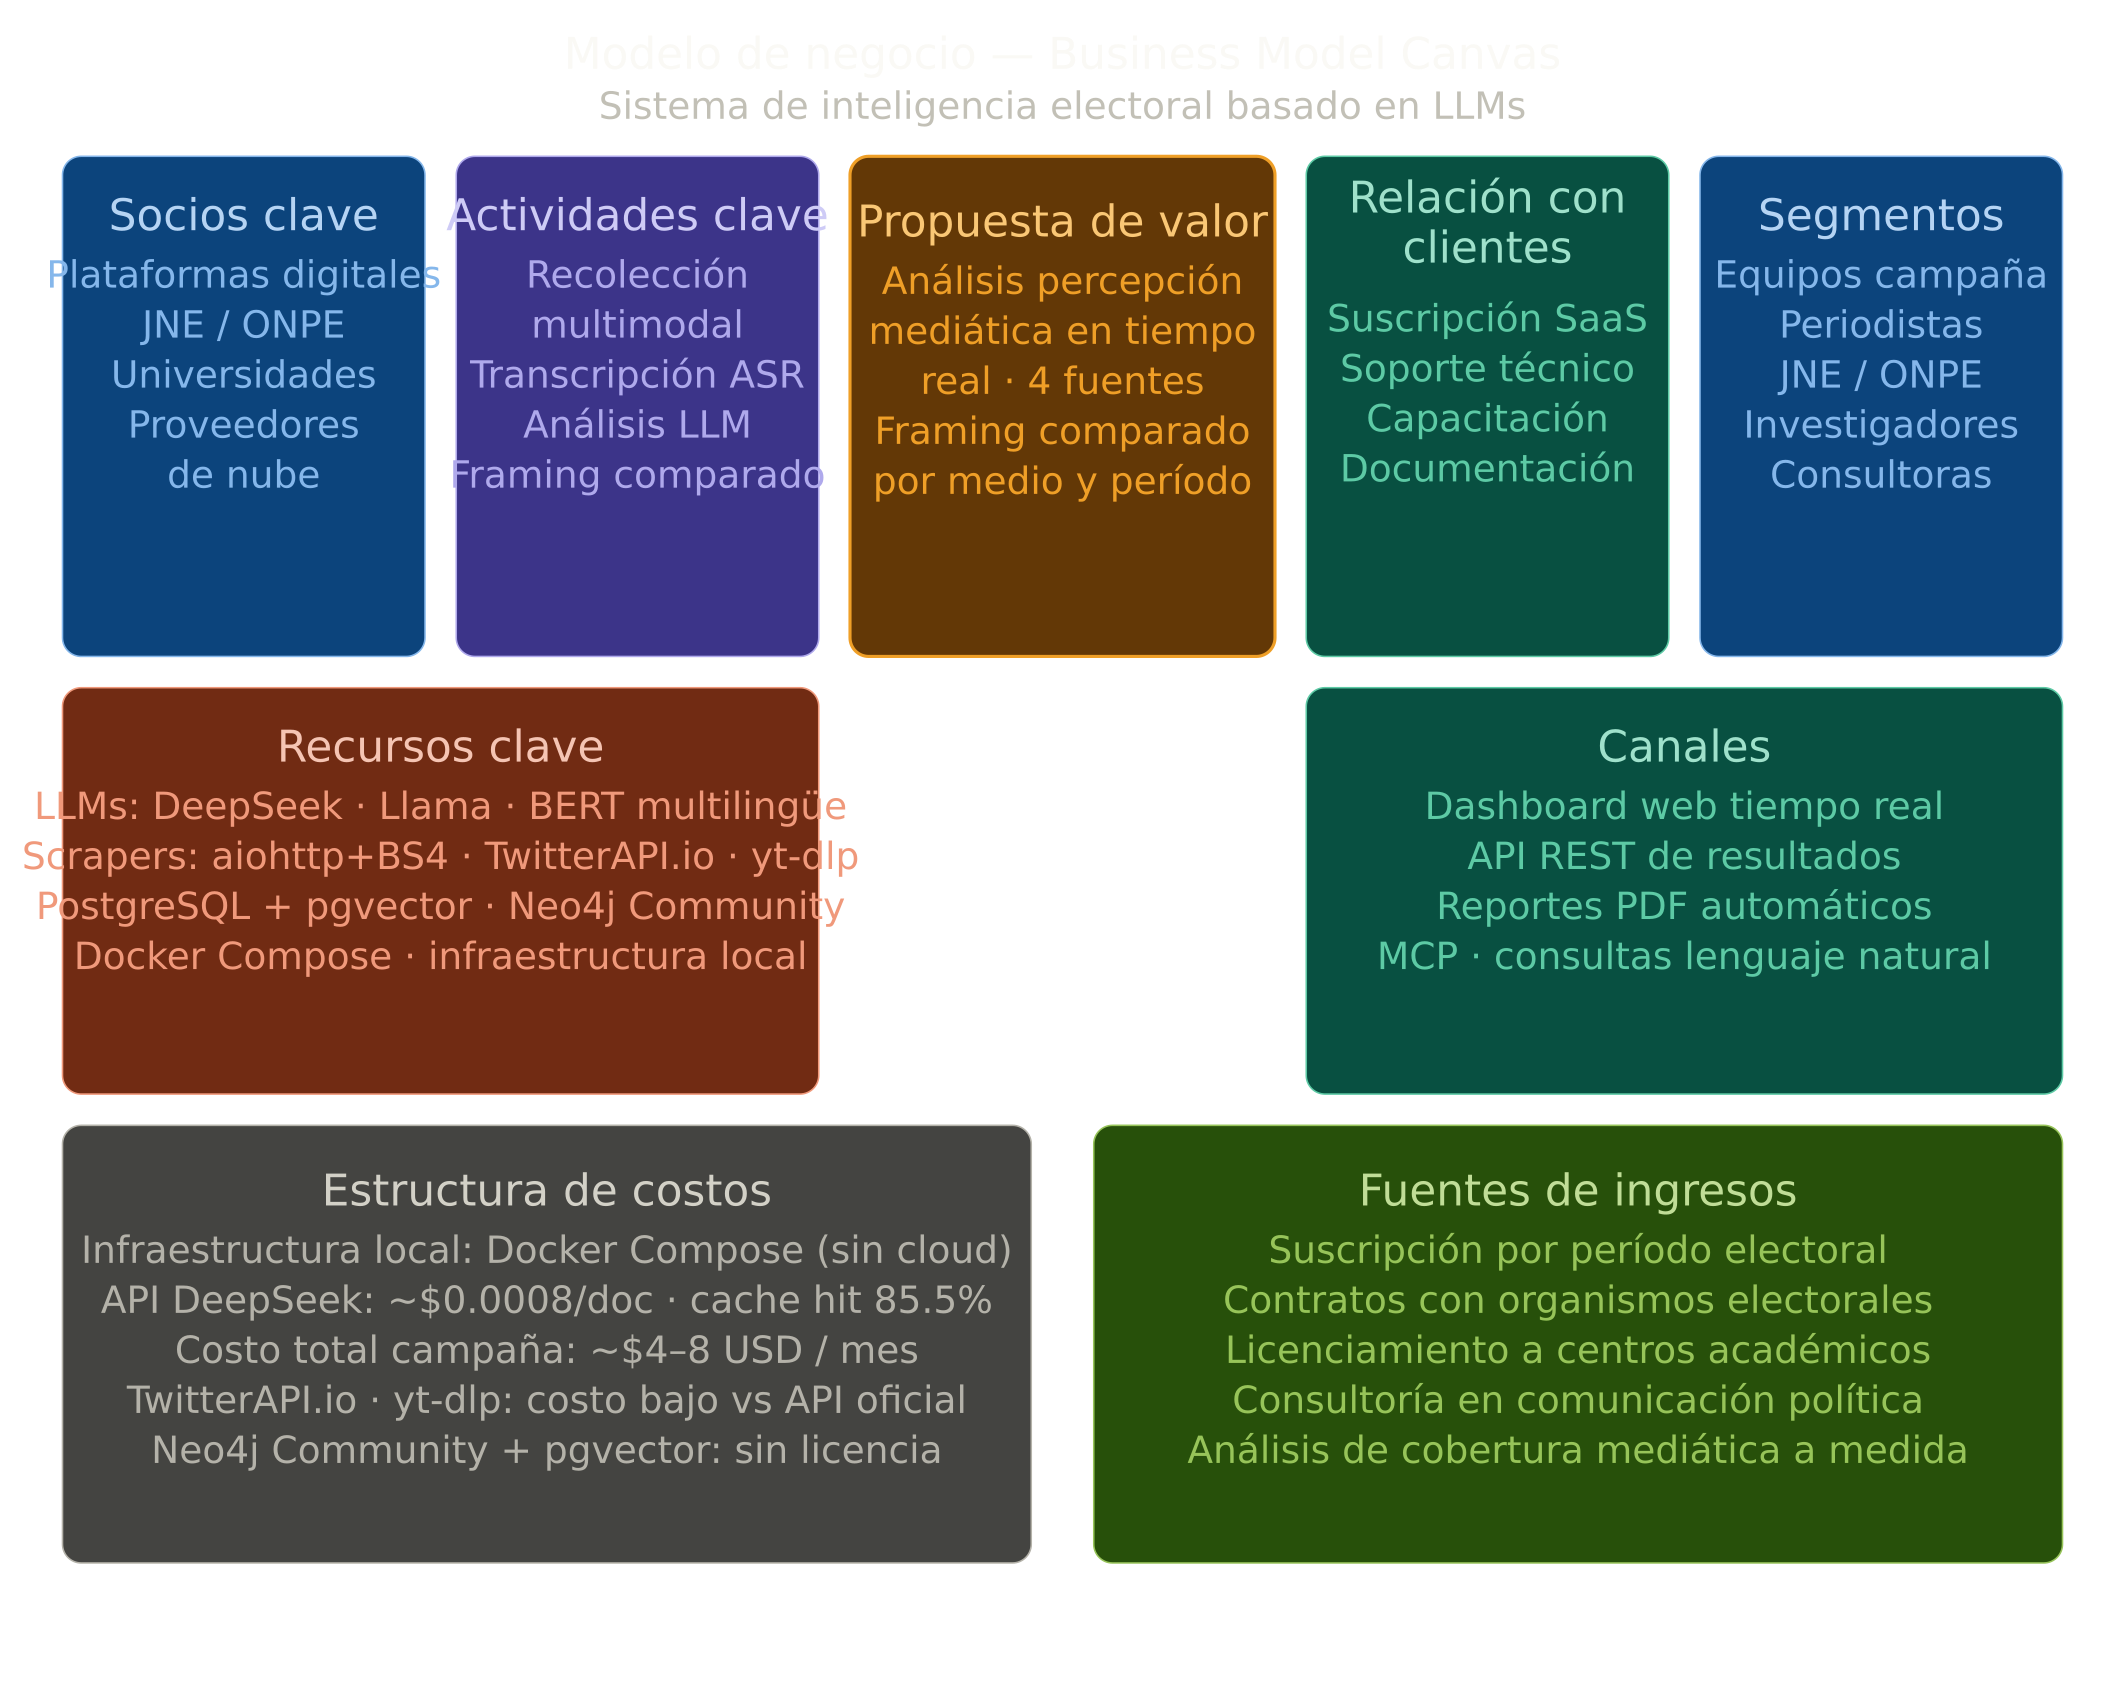
\includegraphics[width=0.92\textwidth]{2.5/figures/canvas_sistema.png}
        % ► NOTA PARA EL AUTOR: actualiza esta figura para reflejar
        %   la propuesta de valor centrada en "percepción proyectada por
        %   los medios" y las 4 fuentes en Recursos Clave. Ver notas_figuras.tex.
        \caption[Modelo CANVAS del sistema de inteligencia electoral basado en LLMs]{Modelo de negocio CANVAS del sistema de inteligencia electoral, mostrando la propuesta de valor centrada en el análisis de percepción mediática, segmentos de clientes, canales, recursos clave (4 fuentes multimodales), actividades clave y estructura de costos.\\
            Fuente: Elaboración propia.}
        \label{fig:canvas_sistema}
    \end{center}
\end{figure}

\section{Mapa de procesos actual}

\subsection{Descripción de los procesos}

El mapa de procesos del sistema de inteligencia electoral se estructura en tres niveles: procesos estratégicos, procesos operativos y procesos de soporte, cuya interacción se ilustra en la Figura \ref{fig:mapa_procesos}. Esta arquitectura de procesos garantiza que el flujo de datos —desde la recolección multimodal hasta la presentación de los indicadores de percepción mediática— sea continuo, trazable y de alta calidad.

\begin{figure}[!ht]
    \begin{center}
        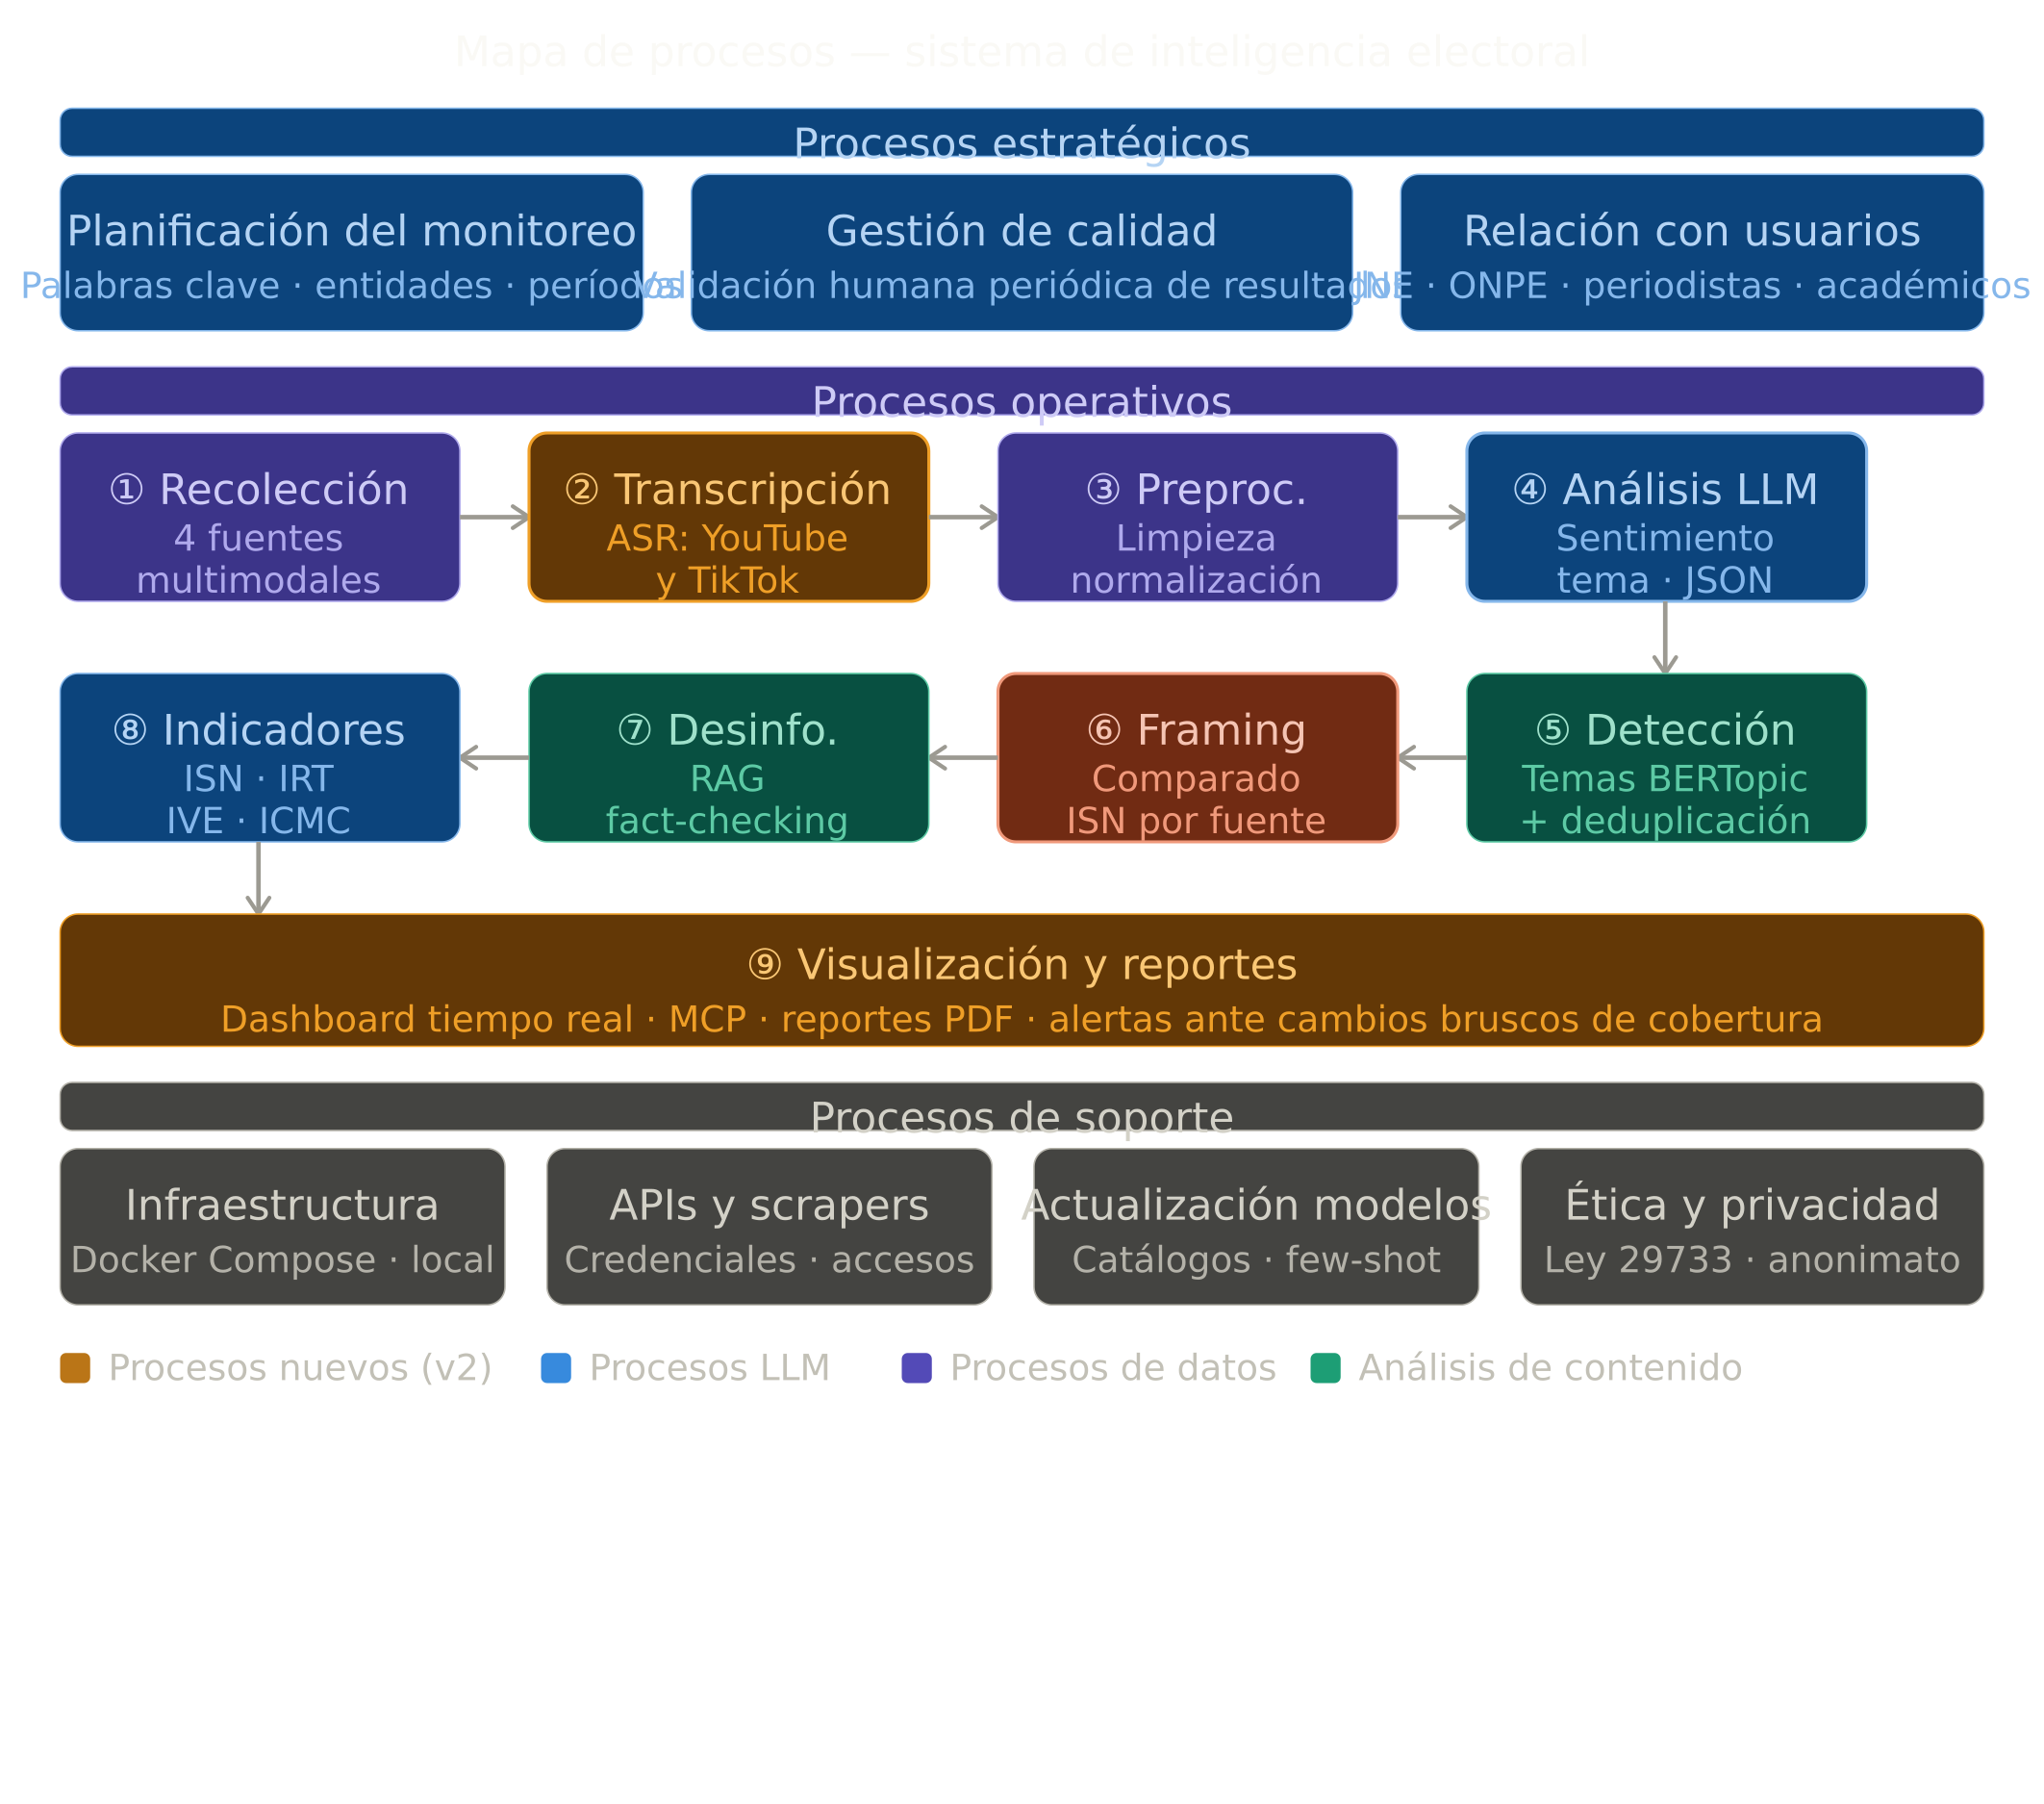
\includegraphics[width=0.95\textwidth]{2.5/figures/mapa_procesos.png}
        % ► NOTA PARA EL AUTOR: actualiza esta figura para incluir
        %   la transcripción audiovisual (YouTube/TikTok) como proceso
        %   operativo y el análisis de framing comparado como salida.
        %   Ver notas_figuras.tex.
        \caption[Mapa de procesos del sistema de inteligencia electoral multimodal]{Mapa de procesos del sistema de inteligencia electoral: procesos estratégicos de planificación y gestión de calidad, procesos operativos del pipeline multimodal (recolección, transcripción, análisis LLM, detección de temas, framing comparado) y procesos de soporte tecnológico y ético.\\
            Fuente: Elaboración propia.}
        \label{fig:mapa_procesos}
    \end{center}
\end{figure}

Los \textbf{procesos estratégicos} incluyen la planificación del monitoreo electoral (definición de palabras clave, medios a monitorear, períodos de análisis y entidades de interés), la gestión de la calidad de los resultados mediante validación humana periódica, y la gestión de las relaciones con los organismos electorales y los usuarios finales del sistema.

Los \textbf{procesos operativos} constituyen el núcleo del sistema y comprenden las siguientes etapas secuenciales:

\begin{itemize}
    \item \textbf{Recolección multimodal de datos}: Ingesta de artículos de noticias mediante scrapers aiohttp + BeautifulSoup de ocho portales; publicaciones de X/Twitter mediante TwitterAPI.io; videos y transcripciones de YouTube; y publicaciones y metadata de TikTok, todo ello filtrado por palabras clave electorales y cuentas de medios relevantes.

    \item \textbf{Transcripción de contenido audiovisual}: Conversión automática de audio a texto de los videos de YouTube y TikTok mediante modelos de reconocimiento de voz, generando transcripciones procesables por el LLM.

    \item \textbf{Preprocesamiento y limpieza de texto}: Eliminación de spam, duplicados y contenido irrelevante; normalización del texto en español (eliminación de URLs, menciones y caracteres especiales); detección de idioma y filtrado de publicaciones en español; almacenamiento en capa Bronze de la arquitectura Medallion.

    \item \textbf{Análisis de sentimientos y framing con LLM}: Clasificación de la polaridad (positivo / negativo / neutral), la emoción y el encuadre mediático de cada documento hacia las entidades políticas mencionadas, mediante prompts diseñados para el contexto de cobertura mediática electoral peruana en modalidad zero-shot y few-shot. La salida se almacena en capa Silver en formato JSON estructurado con campos para: fuente mediática, tipo de plataforma, candidato protagonista, actores secundarios, tema emergente, categoría, sentimiento por candidato y nivel de confianza.

    \item \textbf{Detección dinámica de temas}: Generación de embeddings semánticos con Sentence-BERT multilingüe, construcción de un menú de temas candidatos mediante retrieval multinivel (trending, semántico, léxico, por actor y por evento) y clasificación con LLM en categorías \textit{exact}, \textit{alias} o \textit{new} dentro de un catálogo incremental, con consolidación y deduplicación semántica diaria. La deduplicación entre fuentes heterogéneas se realiza mediante el pipeline de tres etapas descrito en el marco teórico.

    \item \textbf{Análisis de cobertura mediática comparada}: Cálculo del Índice de Sentimiento Neto (ISN) desagregado por fuente mediática y plataforma, identificación de divergencias de framing entre medios y construcción de los perfiles de cobertura por candidato y período.

    \item \textbf{Detección de desinformación}: Verificación automática de los contenidos con mayor viralidad mediante técnicas de RAG, confrontando el contenido con fuentes verificadas y bases de datos de fact-checking.

    \item \textbf{Cálculo de indicadores y generación de reportes}: Cómputo del ISN, IRT, IVE e ICMC por entidad política, fuente mediática y período de tiempo; generación automática de reportes diarios y alertas ante cambios bruscos de cobertura. Los resultados se materializan en vistas Gold de la arquitectura Medallion.
\end{itemize}

Los \textbf{procesos de soporte} incluyen la gestión de la infraestructura tecnológica local (Docker Compose), el monitoreo del rendimiento de los modelos LLM, la gestión de las credenciales y permisos de las APIs y scrapers, el mantenimiento y actualización de los catálogos de entidades electorales, y la supervisión ética y de privacidad de los datos procesados.